\documentclass[french]{article}
\usepackage{babel}
\usepackage[T1]{fontenc}
\usepackage[utf8]{inputenc}
\usepackage{listings}
\usepackage{color}
\usepackage{listingsutf8}
\usepackage{graphicx}

\title{boo-climb}
\author{CoderDojo Ans}
\date{Décembre 2018}
\graphicspath{ {./Images/} }

\definecolor{codegreen}{rgb}{0,0.6,0}
\definecolor{codegray}{rgb}{0.5,0.5,0.5}
\definecolor{codepurple}{rgb}{0.58,0,0.82}
\definecolor{backcolour}{rgb}{0.95,0.95,0.92}

\lstdefinestyle{mystyle}{
	backgroundcolor=\color{backcolour},   
	commentstyle=\color{codegreen},
	keywordstyle=\color{magenta},
	numberstyle=\tiny\color{codegray},
	stringstyle=\color{codepurple},
	basicstyle=\footnotesize,
	breakatwhitespace=false,         
	breaklines=true,                 
	captionpos=b,                    
	keepspaces=true,                 
	numbers=left,                    
	numbersep=5pt,                  
	showspaces=false,                
	showstringspaces=false,
	showtabs=false,                  
	tabsize=2,
	literate=
	{á}{{\'a}}1 {é}{{\'e}}1 {í}{{\'i}}1 {ó}{{\'o}}1 {ú}{{\'u}}1
	{Á}{{\'A}}1 {É}{{\'E}}1 {Í}{{\'I}}1 {Ó}{{\'O}}1 {Ú}{{\'U}}1
	{à}{{\`a}}1 {è}{{\`e}}1 {ì}{{\`i}}1 {ò}{{\`o}}1 {ù}{{\`u}}1
	{À}{{\`A}}1 {È}{{\'E}}1 {Ì}{{\`I}}1 {Ò}{{\`O}}1 {Ù}{{\`U}}1
	{ä}{{\"a}}1 {ë}{{\"e}}1 {ï}{{\"i}}1 {ö}{{\"o}}1 {ü}{{\"u}}1
	{Ä}{{\"A}}1 {Ë}{{\"E}}1 {Ï}{{\"I}}1 {Ö}{{\"O}}1 {Ü}{{\"U}}1
	{â}{{\^a}}1 {ê}{{\^e}}1 {î}{{\^i}}1 {ô}{{\^o}}1 {û}{{\^u}}1
	{Â}{{\^A}}1 {Ê}{{\^E}}1 {Î}{{\^I}}1 {Ô}{{\^O}}1 {Û}{{\^U}}1
	{œ}{{\oe}}1 {Œ}{{\OE}}1 {æ}{{\ae}}1 {Æ}{{\AE}}1 {ß}{{\ss}}1
	{ű}{{\H{u}}}1 {Ű}{{\H{U}}}1 {ő}{{\H{o}}}1 {Ő}{{\H{O}}}1
	{ç}{{\c c}}1 {Ç}{{\c C}}1 {ø}{{\o}}1 {å}{{\r a}}1 {Å}{{\r A}}1
	{€}{{\EUR}}1 {£}{{\pounds}}1
}

\lstset{
	style=mystyle, 
	inputencoding=utf8/latin9
}

\newcommand{\tips}{
\includegraphics[scale=0.08]{tips}\textbf{\textit{Astuces\\}}}

\newcommand{\todo}{
\includegraphics[scale=0.1]{work_in_progress}\textbf{ A vous de jouer\\} }

\newcommand{\result}{
\includegraphics[scale=0.1]{green_tick}\textbf{Vérification\\}}


\begin{document}

\begin{titlepage}
	\maketitle
\end{titlepage}

\tableofcontents{}
\newpage

\section{Mise en place de l'environnement}

\begin{abstract}
	Dans cette section, nous allons mettre en place l'environnement et le décor du jeu.
\end{abstract}
	
\subsection{Le canevas de départ}	

\lstinputlisting[language=Python]{Codes/Step1.py}

Ce qui devrait donner la situation suivante\\

\begin{center}
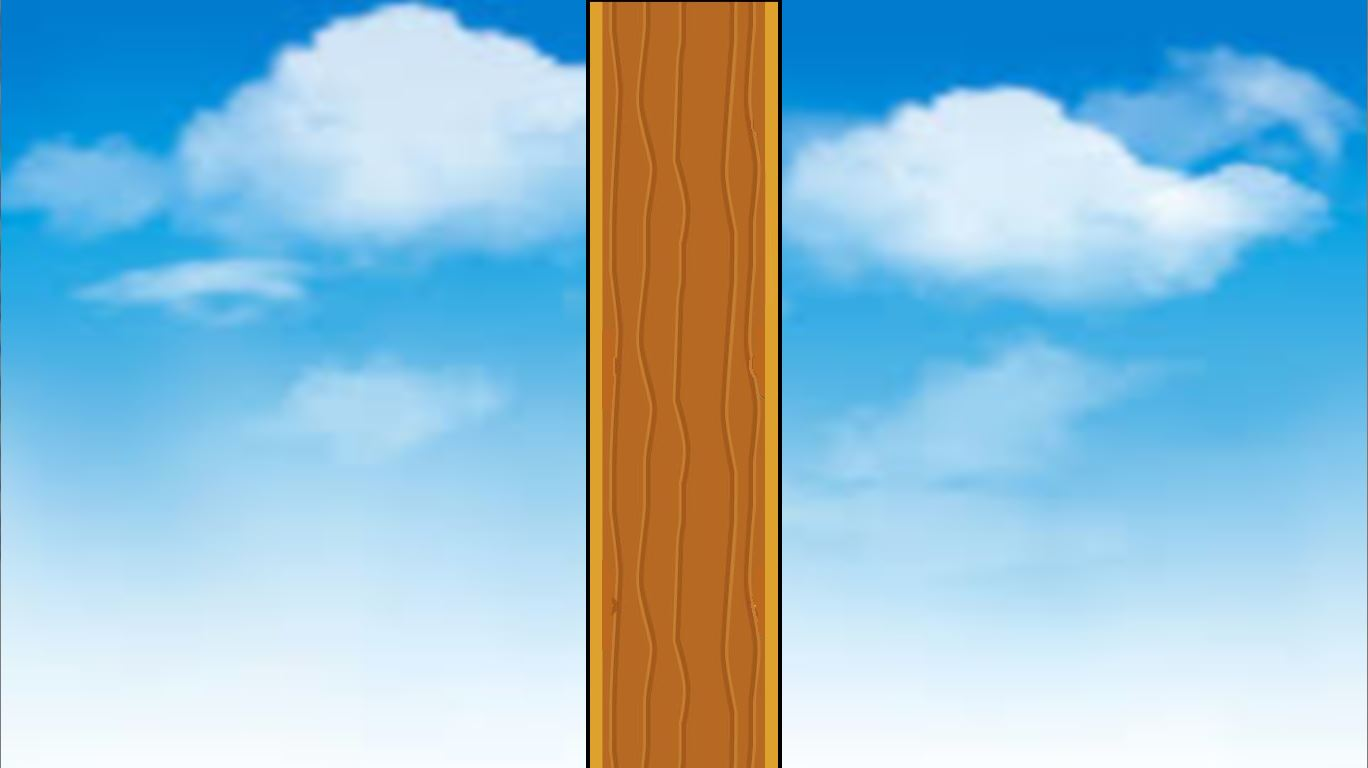
\includegraphics[scale=0.20]{step1}
\end{center}
	
\newpage
	
\subsection{Placer les branches et le boo}	
	
Dans le répertoire "images" fourni, on peut trouver plusieurs types de branches, un personnage (boo), ainsi qu'une bombe. Dans un premier temps, pour faire plus simple, nous n'allons utiliser que les branches en bon état et le personnage tel que ci-dessous.	
	
\begin{center}
	
\includegraphics[scale=2]{boo}
	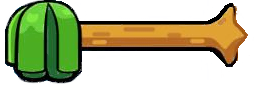
\includegraphics[scale=0.5]{good_branch_left}
	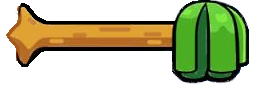
\includegraphics[scale=0.5]{good_branch_right}
\end{center}	

\tips

Afin d'obtenir un bon rendu visuel et de faciliter les animations futures, il est important que les branches soit espacées de manière équidistantes ! Le plus simple consiste donc à en placer une de chaque côté et de créer les autres via une boucle. Pour utiliser efficacement les boucles, les listes sont généralement d'une aide précieuse. Le code d'exemple ci-dessous montre comment les utiliser.	

\lstinputlisting[language=Python]{Codes/Step2.py}
	
\todo 

\begin{enumerate}
\item Placer de chaque côté de l'arbre 4 branches à droite et à gauche. 
\item Positionner le personnage sur la branche la plus basse à droite.\\

\end{enumerate}

\result

A la fin de cette étape vous devriez avoir le résultat suivant.

\begin{center}
	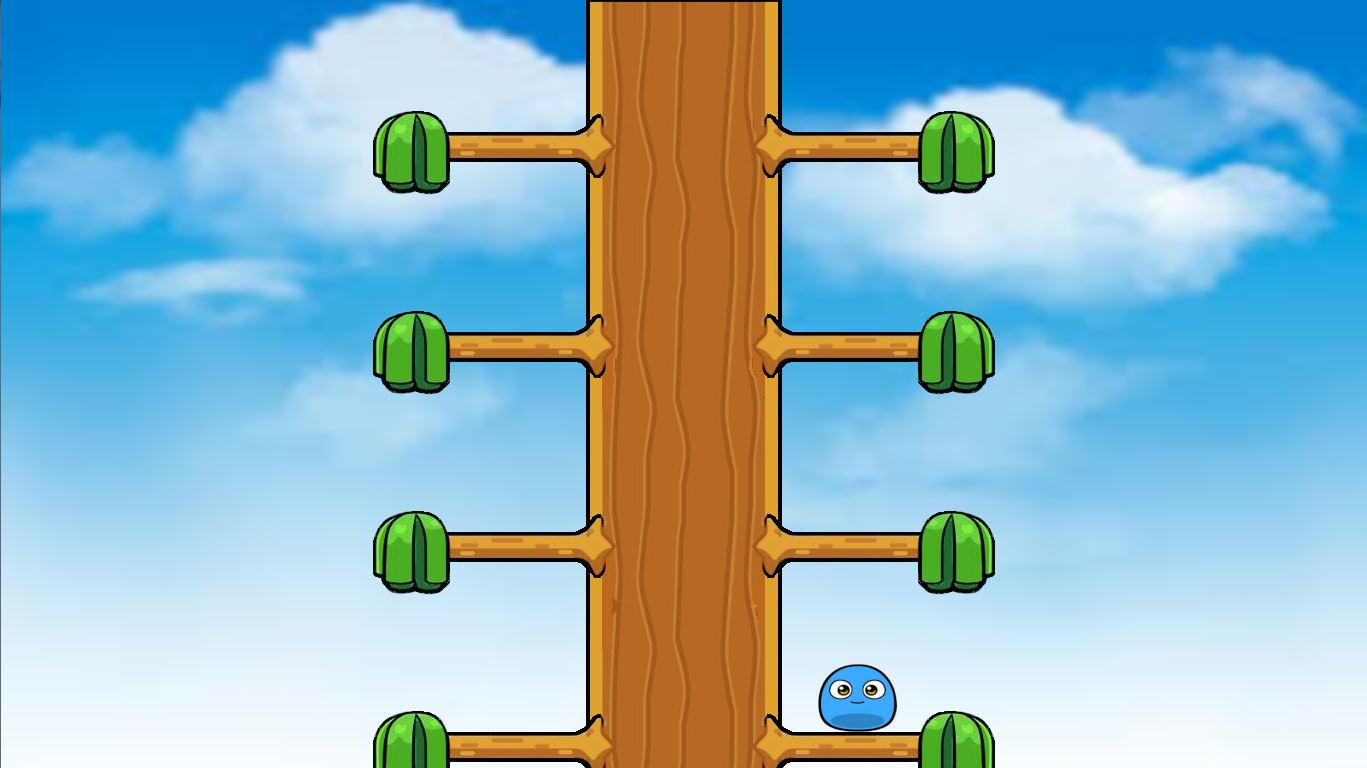
\includegraphics[scale=0.20]{step2}
\end{center}

\section{Les animations}
	
\begin{abstract}
	Dans cette section, nous allons faire les animations du personnage et des branches.\\
	
	Le but est de faire en sorte que le boo saute de branche en branche. Pour ce faire, à chaque fois que l'utilisateur déclenche une action, nous allons déplacer le boo latéralement au besoin et les branches verticalement.  
\end{abstract}
	
\subsection{Déplacer le boo}	
	
Le jeu ne comporte que 2 touches : $\leftarrow$ et $\rightarrow$.\\ 

Pour faire simple, nous allons uniquement le déplacer latéralement (i.e. seule la coordonnée x change). Il n'y a donc que 4 combinaisons possibles :

\begin{enumerate}
	\item Le boo est à gauche et on veut aller à gauche
	\item Le boo est à gauche et on veut aller à droite
	\item Le boo est à droite et on veut aller à gauche
	\item Le boo est à droite et on veut aller à droite
\end{enumerate}	

Par conséquent, il n'y a réellement que 2 combinaisons (2 et 3) où le boo doit bouger qui sont représentées ci-dessous !

\begin{center}
	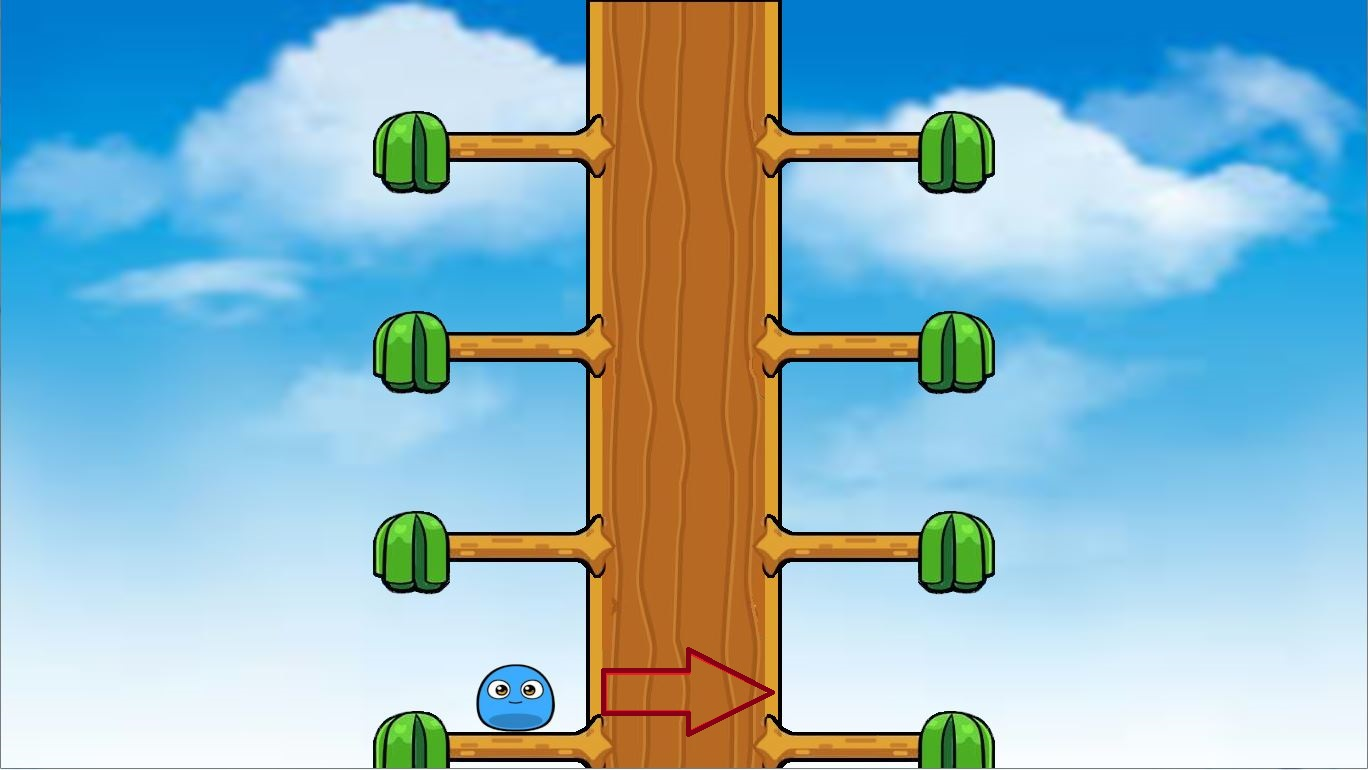
\includegraphics[scale=0.20]{step3-1}
	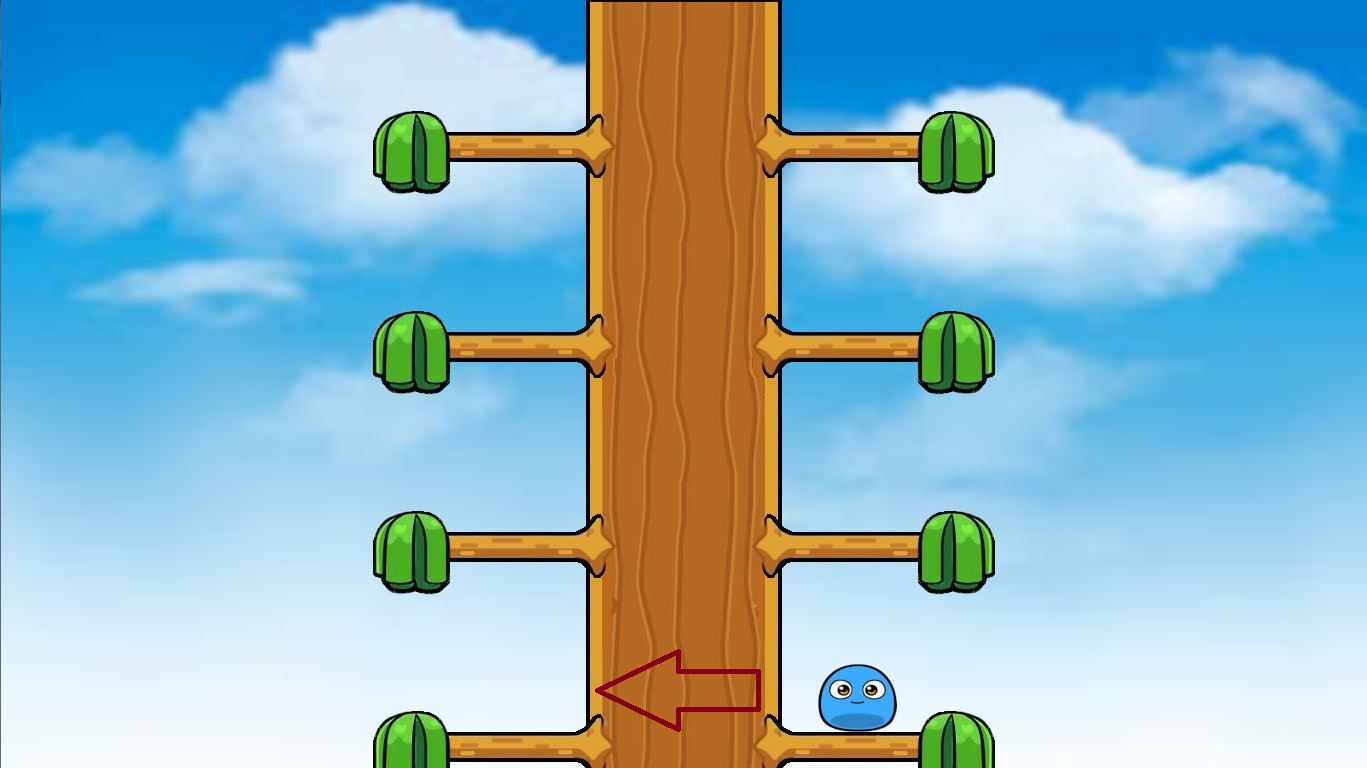
\includegraphics[scale=0.20]{step3-2}
\end{center}

\tips

\begin{enumerate}
	\item Si X1 désigne la position de départ du boo et X2 la position d'arrivée, on peut calculer le déplacement à effectuer comme étant X = X2 - X1\\
	
	\item Une fois qu'on connait cet écart X, il faut pouvoir déplacer le personnage progressivement pour donner l'impression d'un mouvement fluide. Pour ce faire, la fonction \textbf{\textit{update()}} est toute indiquée. Comme l'indique la documentation, celle-ci est appelée 60 fois par seconde. Comme on peut le voir sur le schéma ci-dessous, on peut donc calculer le temps T qui s'écoule entre 2 appels successifs : \\
	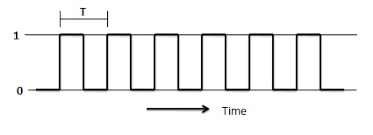
\includegraphics[scale=0.8]{horloge}
	\[T = \frac{1}{60} = 0.01666s = 16,6 ms\] 
	
	
	Pour donner un exemple chiffré, si X = 60 pixels et qu'on déplace le boo d'un pixel à la fois par fonction update (e.g. boo.x += 1), il faudra 1s au boo pour atteindre sa destination. \\
	
	\item Finalement, il reste à pouvoir déterminer quand l'animation commence et quand elle s'arrête pour savoir quand exécuter du code dans la fonction update et quand ne pas le faire.\\
	
	En mettant tout ça en musique, on obtient à peu près le canevas de départ suivant :
	\lstinputlisting[language=Python]{Codes/Step3.py}
	
\end{enumerate}

\todo

En vous inspirant du code ci-dessus et sur base des astuces, programmer le déplacement du boo sur la gauche ou sur la droite pour les 2 touches.\\

\textbf{Challenge optionnel\\}

Pour les plus courageux d'entre vous, le challenge consiste à faire effectuer un léger déplacement vertical aller/retour (sur la composante Y) au boo durant son déplacement latéral comme illustré ci-dessous. Cela donnera un plus bel effet de saut.\\

\begin{center}
	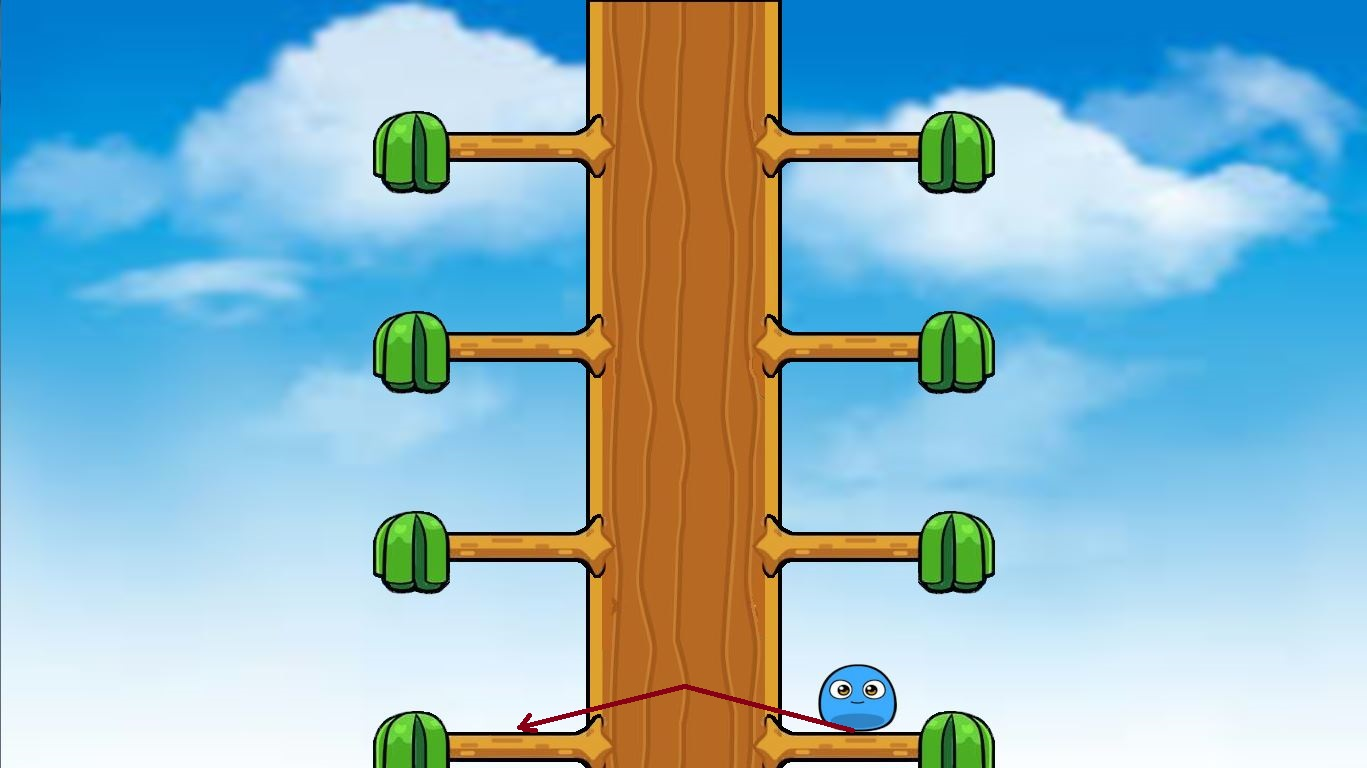
\includegraphics[scale=0.20]{step3-3}
\end{center}

\result

A la fin de cette étape, le boo devrait pouvoir se déplacer de gauche à droite suivant sa position et les touches sur lesquelles on appuye.

\subsection{Déplacer les branches}

Notre boo bouge mais puisque les branches sont toujours immobiles, on a pas l'impression qu'il saute réellement. Nous allons donc y remédier en faisant bouger les branches aussi.\\

Le principe reste le même, lorsque l'utilisateur appuye sur une de 2 touches citées précédemment, on déclenche l'animation des branches. Pour ce faire, chacune de celles-ci va descendre pour finalement atteindre la position qu'occupait précédemment la branche du dessous.\\

La logique est donc exactement la même que celle qu'on a employée pour faire se déplacer le boo. La différence c'est que, cette fois, seule la composante Y importe et qu'il y a plus qu'une branche.

\begin{center}
	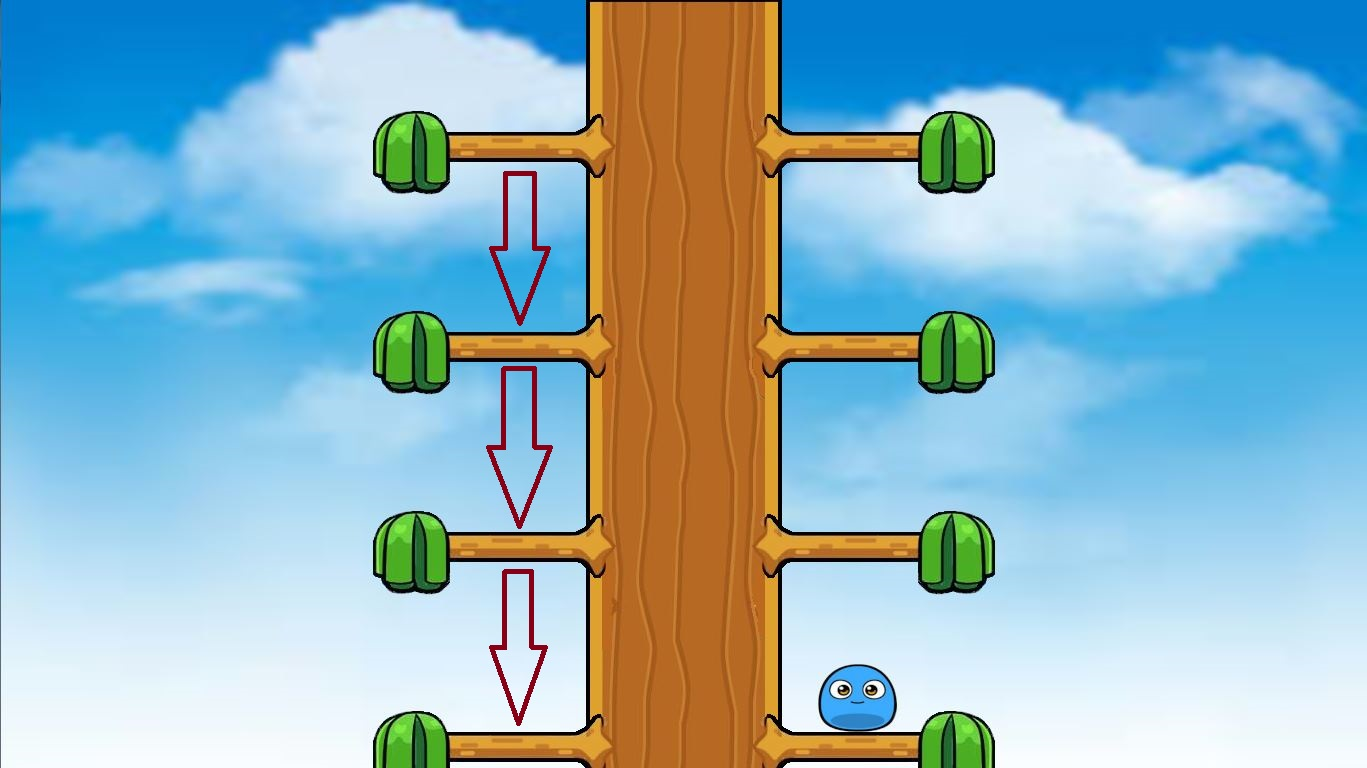
\includegraphics[scale=0.20]{step4-1}
\end{center}

\tips

\begin{enumerate}

\item A mesure que les branches descendent, il doit en apparaître une nouvelle dans le dessus de l'écran. Si le code a été bien structuré avec des boucles dès le départ, ajouter une branche supplémentaire qui se trouve initialement en dehors de l'écran ne devrait pas poser de problème.\\

\item Une fois que les branches sont descendues et ont terminé leur animation, chaque branche s'est déplacée d'une position vers le bas. En terme algorithmique, si on considère que la branche la plus haute est la branche 0, la suivante la branche 1, etc, ... On peut considérer qu'on arrive à la situation suivante :

\end{enumerate}

\begin{center}
	\begin{tabular}{lll}
	  & Avant & Après\\	
	0 & B0 & Nouvelle branche\\
	1 & B1 & B0\\
	2 & B2 & B1\\
	3 & B3 & B2\\
	4 & B4 & B3\\
	\end{tabular}
\end{center}

Il faut donc repositionner chaque élément dans la liste et le tour est joué !\\

\todo

Ecrivez le code pour déplacer les branches en vous inspirant de ce que vous avez fait pour déplacer le boo.\\

\result

 Vous devriez maintenant avoir un personnage qui, en fonction des touches enfoncées, saute de branche en branche dans l'arbre. Le déplacement cumulé du personnage et des branches doit donner l'illusion que le boo monte bel et bien dans l'arbre.

\subsection{Faire disparaître certaines branches}

Jusqu'à présent nous avons toujours afficher toutes les branches de chaque côté de l'arbre. Cela nous à permis de nous assurer que les animations fonctionnaient correctement. Néamoins, pour que le jeu présente un intérêt, il est important qu'il y ait parfois des branches manquantes de certains côtés sans quoi il est tout simplement impossible de perdre !

\begin{center}
	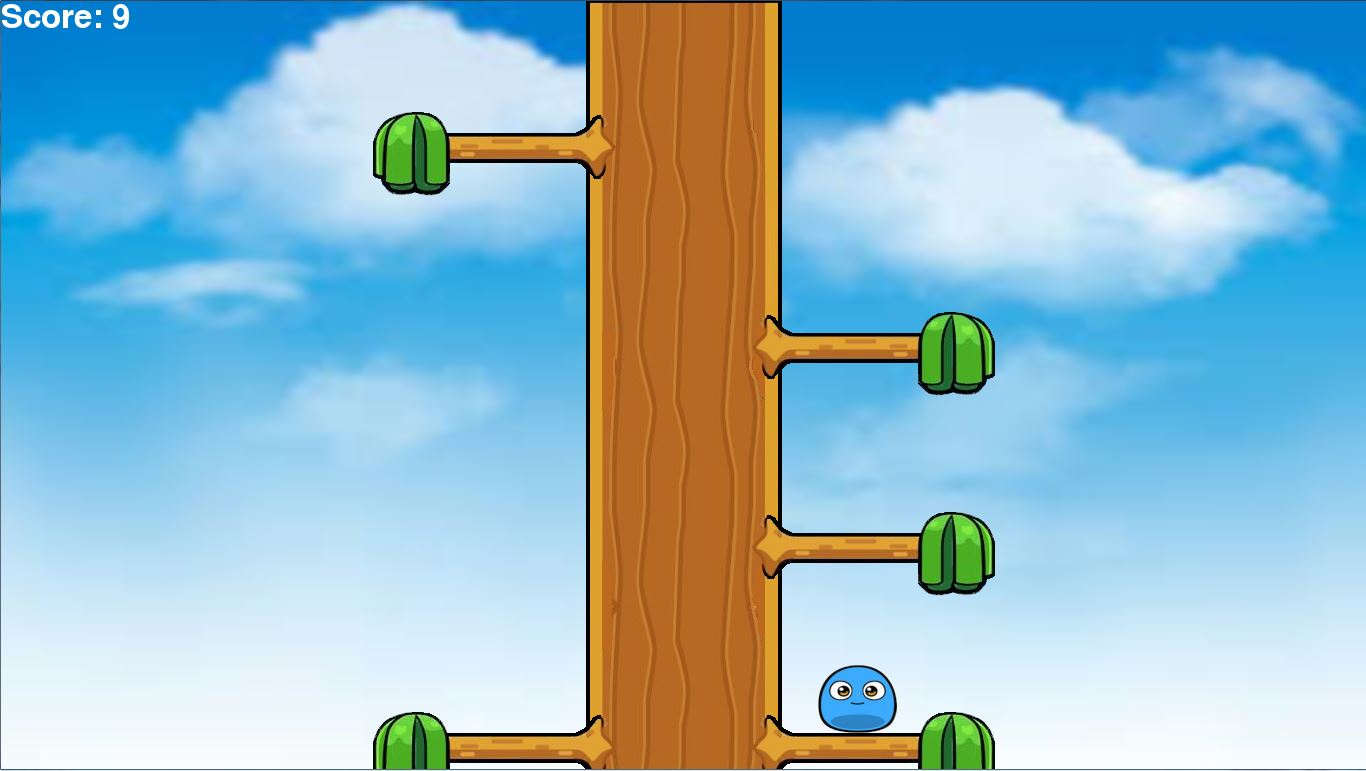
\includegraphics[scale=0.20]{Image_4}
\end{center}

\tips

\begin{enumerate}

\item Il ne peut jamais y avoir 2 branches manquantes sur le même étage, sans quoi il est impossible d'aller plus haut ! Il n'y a donc au total que 3 possibilités (les 2 branches sont là, seule la branche de gauche est là, seule la branche de droite est là)\\

\item Pour faire "disparaître" un élément, le plus simple est tout simplement de ne pas le dessiner. Il est également possible en Python de dire qu'un élément n'existe pas. On peut par conséquent vérifier si l'élément existe avant d'effectuer une action sur ce dernier.

\begin{center}
	\lstinputlisting[language=Python]{Codes/Step4.py}
\end{center}
 
\item Finalement, pour que le jeu soit plaisant et différent à chaque fois, il est important de faire apparaître aléatoirement les branches. L'exemple suivant montre comment générer un nombre aléatoire en Python 

\begin{center}
	\lstinputlisting[language=Python]{Codes/Step5.py}
\end{center}

\end{enumerate}

\todo

Programmer la logique qui fait apparaître les nouvelles branches pour que, de manière aléatoire, il n'y ait pas toujours 2 branches de chaque côté de l'arbre.\\

\result

A la fin de cette étape votre boo est capable de grimper de branche en branche. A chaque fois qu'il saute de nouvelles branches apparaissent suivant un ordre imprévisible.

\section{La logique du jeu}

\begin{abstract}
	Nous avons jusqu'à présent programmé tous les éléments visibles. Cependant, il n'est toujours pas possible à ce stade ni de gagner, ni de perdre. En effet, même si votre personnage saute du côté où il n'y a pas de branche, rien ne se passe. Il est donc à présent temps de passer à la logique opérationnelle du jeu elle-même
\end{abstract}

\subsection{Comptabiliser les points}

Comme dans tout jeu qui se respecte un compteur avec des points est toujours sympathique. Pour ce faire, on peut compter chaque fois que le boo parvient à sauter sur une branche valide.\\

Idéalement le score devrait être affiché à l'écran.\\

\tips

\begin{enumerate}

\item Penser à bien initialiser le score à 0 en début de partie.

\item N'incrémenter le score qu'à la fin de chaque animation réussie\\

\end{enumerate}	

\todo

Ajouter et afficher le score du jeu.\\

\result

Vous devriez à présent avoir un personnage qui est capable de monter de branche en branche avec un score qui représente le nombre de saut réussi. 

\subsection{Perdre le jeu}

Le jeu est perdu lorsque le boo saute d'un côté où il n'y a pas de branche. Au vu de tout ce que vous avez déjà fait, il ne devrait pas être trop compliqué de détecter cette situation.\\

\tips

\begin{enumerate}
	
\item Le boo ne peut se trouver qu'à 2 positions qui correspondent toujours au même niveau sur l'arbre. Il suffit donc de regarder, en fin d'animation, si la branche où il se trouve est visible ou pas\\

\item Dans le cas où le jeu est perdu, puisqu'il n'y a plus de branche, prévoir une animation où le boo tombe jusqu'à sortir de l'écran serait du plus bel effet.\\
	
\end{enumerate}	

\todo

Détecter que le boo a sauté d'un côté ou il n'y a plus de branche. Le faire tomber hors de l'écran et afficher un texte qui dit "Game over". 

\subsection{Redémarrer le jeu}

Une fois que le jeu est perdu, l'utilisateur aura peut-être à coeur de refaire une partie. Il serait donc souhaitable qu'il puisse redémarrer le jeu immédiatement sans avoir à le quitter et le redémarrer.\\

\tips

\begin{enumerate}
	
	\item Choisir une touche pour faire redémarrer le jeu (exemple : ENTER ou bien n'importe quelle touche)\\
	
	\item Il ne faut redémarrer le jeu que s'il est perdu\\
	
	\item Tout le code est déjà là mais il faut peut-être probablement le remettre dans des fonctions pour éviter de le dupliquer\\
	
\end{enumerate}	

\todo

Une fois le jeu perdu, permettre à l'utilisateur de redémarrer une nouvelle partie en appuyant sur une touche.\\

\result

Ca y est ! Vous avez une première version d'un jeu tout à fait jouable. Félicitations ! 

\section{Pour aller plus loin}

\subsection{Challenge 1 : ajouter des bombes}

Les images fournies contiennent une bombe. 

\begin{center}
	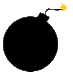
\includegraphics[scale=2]{bomb}
\end{center}

Pour pimenter le jeu, on pourrait aléatoirement ajouter des bombes sur certaines branches. Le jeu serait alors également perdu si le boo venait à sauter sur une branche avec une bombe.\\

\tips

\begin{enumerate}
	
	\item Il ne peut y avoir de bombes que lorsque les branches sont présentes de chaque côté de l'arbre\\
	
	\item Il faut animer les bombes de la même manière que les branches.\\
	
	\item Il faut détecter la présence des bombes de la manière que les branches\\
	
\end{enumerate}	

\subsection{Challenge 2 : ajouter des branches qui cassent}

Les images contiennent également des branches abîmées.

\begin{center}
	
\includegraphics[scale=0.5]{bad_branch_left}
	
\includegraphics[scale=0.5]{bad_branch_right}
\end{center}	

Ce qui pourrait rajouter encore plus de défi pour l'utilisateur c'est d'intégrer des branches abîmées. Le principe d'une branche abîmée étant qu'on peut sauter dessus mais qu'on ne peut pas y rester trop longtemps sous peine qu'elle se casse !\\

\tips

\begin{enumerate}
	
	\item La branche cassée est à priori une branche comme les autres. C'est juste l'image qui est différente. On peut donc savoir en inspectant la propriété \textbf{\textit{image}} de l'objet s'il s'agit d'une branche cassée ou non.\\
	
	\item Il faut pouvoir détecter que le boo vient de sauter sur une branche cassée et démarrer un compteur pour comptabiliser le temps qu'il reste dessus (voir 2.1 déplacer le boo).\\
	
	\item Ce compteur doit être remis à zéro à chaque fois que le boo saute à un autre endroit.\\
	
	\item Si le compteur dépasse la valeur d'attente, la branche disparait et se transforme en "pas de branche" : le jeu est perdu.\\

\end{enumerate}

\end{document}
	